
\documentclass[ms.tex]{subfiles} 
\begin{document} 

\section{Introduction} 
\label{sec:intro} 
\begin{itemize} 
	\item In terms of astrophysical nucleosynthesis, nitrogen (N) is a unique 
	element. 
	\begin{itemize} 
		\item It's one of only a few elements lighter than strontium (Z = 38) 
		with significant nucleosynthetic yields from asymptotic giant branch 
		(AGB) stars~\citep{Johnson2019}. 

		\item Alongside helium, it is one of the primary nuclear fusion 
		products of main sequence stars more massive than the sun with nonzero 
		metallicity. 
		The CNO cycle\footnote{
			\Ctwelve(p,$\gamma$)\Nthirteen($\beta^+$,$\nu_e$)\Cthirteen 
			(p,$\gamma$)\Nfourteen(p,$\gamma$)\Ofifteen
			($\beta^+$,$\nu_e$)\Nfifteen(p,$\alpha$)\Ctwelve 
		} catalyses the proton-proton chain of nuclear 
		reactions~\citep*[e.g.][]{Suliga2020} using carbon (C), N, and oxygen 
		(O) target nuclei, the slowest component of which is 
		the~\Nfourteen(p,$\gamma$)\Ofifteen~reaction. 
		This bottleneck is a sufficiently strong effect such that, to first 
		order, the effect of the CNO cycle is to convert all of the C and O 
		isotopes in a star into~\Nfourteen. 

		\item It's among a select group of elements whose observed abundances 
		in stellar spectra often do not reflect the star's birth abundances. 
		Internal mixing processes (particularly dredge-up) changes the 
		surface abundances of C and N in red giants, a phenomenon both expected 
		from theoretical models and observed in open and globular 
		clusters~\citep{Gilroy1989, Korn2007, Lind2008, Souto2018, Souto2019}. 
	\end{itemize} 

\end{itemize}

\begin{figure*} 
\centering 
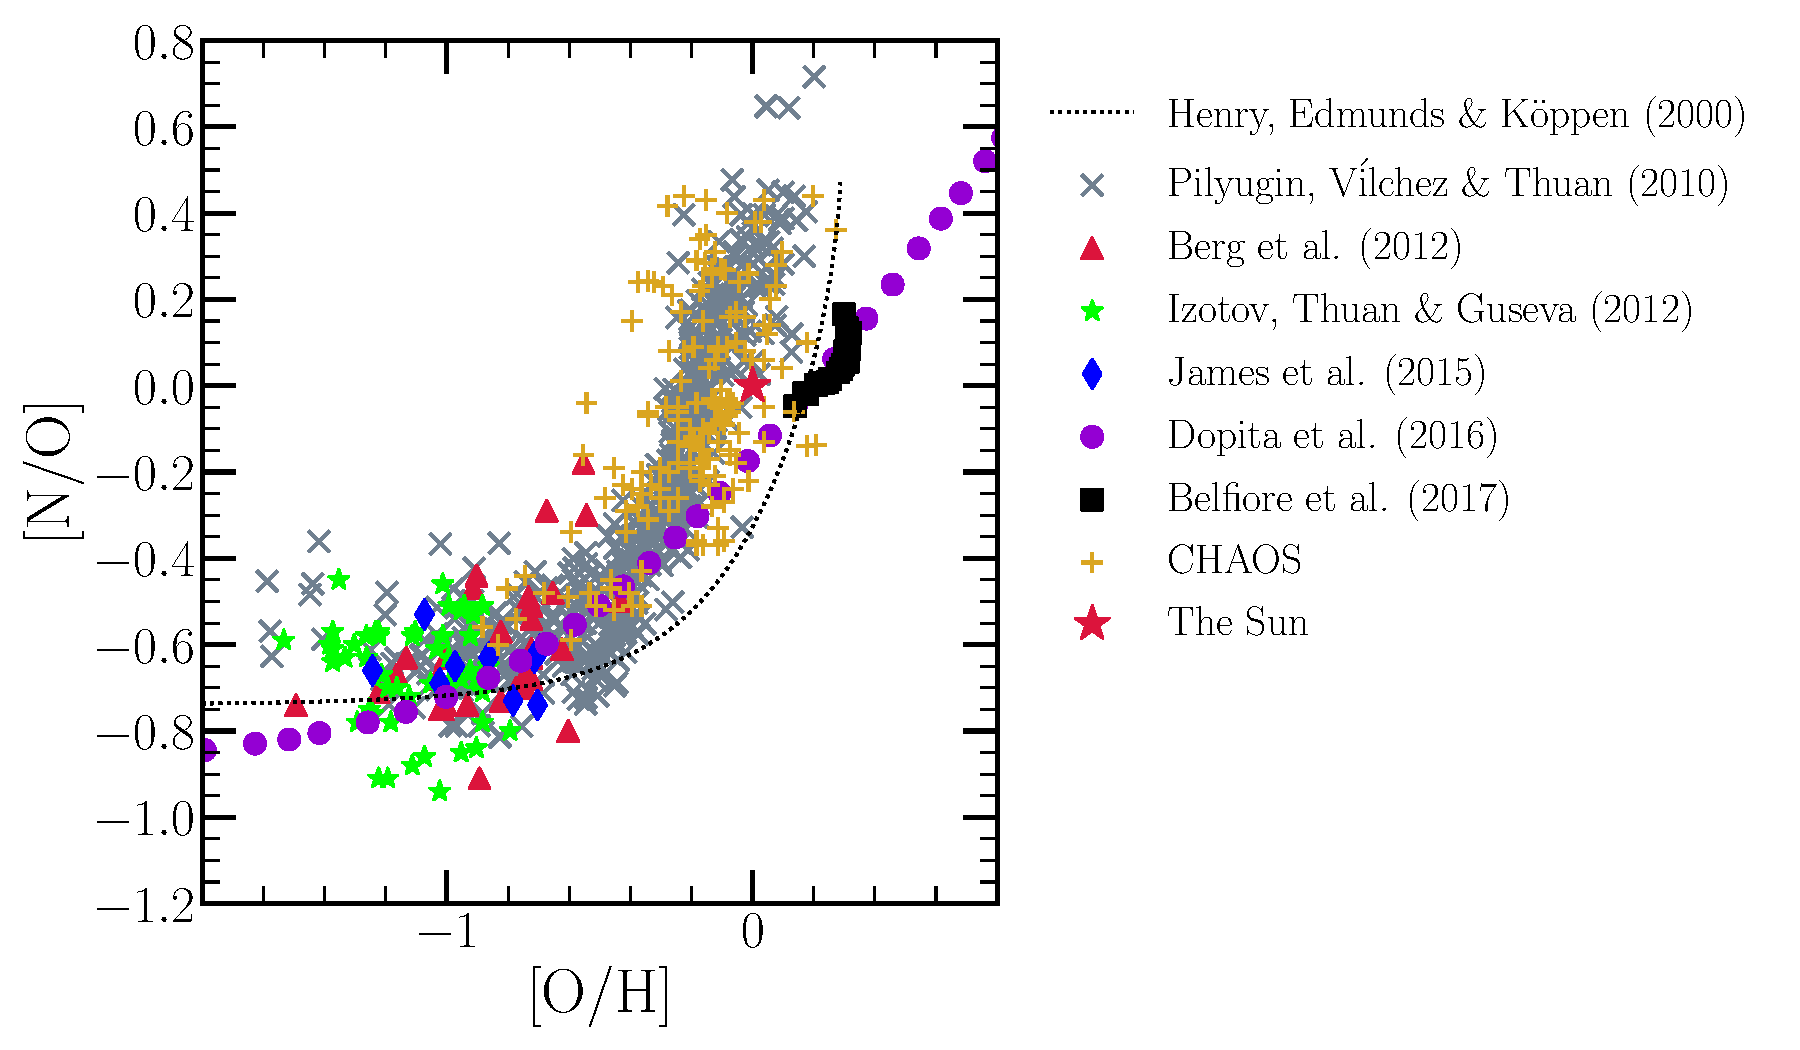
\includegraphics[scale = 0.5]{no_oh_observed.pdf} 
\caption{
The [N/O]-[O/H] relation as observed in different galactic environments:
HII regions from the first six CHAOS galaxies (golden +'s: NGC 3184, NGC 628, 
NGC 5194, NGC 5457, M101, and NGC 2403;~\citealp{Berg2020, Skillman2020,
Rogers2021}) and other nearby NGC spiral galaxies (grey X's:
\citealp*{Pilyugin2010}), HII regions in blue, diffuse star forming dwarf
galaxies (red triangles:~\citealp{Berg2012}; green stars:~\citealp*{Izotov2012};
blue diamonds:~\citealp{James2015}), in local stars and HII regions (purple
circles:~\citealp{Dopita2016}), and in the MaNGA IFU survey (black squares:
\citealp{Belfiore2017}).
The fit to [N/O] as a function of [O/H] in Galactic and extragalactic HII 
regions by~\citet*{Henry2000} is shown in a black dotted line. 
The Sun, at (0, 0) on this plot by definition, is marked by a red star. 
We omit the uncertainties for visual clarity. 
{\color{red} To do: Pull the data Noah Rogers's paper on NGC 2403 and add it
to this figure.
} 
} 
\label{fig:no_oh_observed} 
\end{figure*} 

\begin{itemize} 
	\item Both observationally and theoretically, N is among the more well 
	studied elements. 
	Fig.~\ref{fig:no_oh_observed} presents a compilation of observed abundances 
	of N and O in the gas phase: 
	\begin{itemize} 
		\item HII regions in the first six CHAOS galaxies (NGC 3184, NGC 628,
		NGC 5194, NGC 5457, M101, and NGC 2403;~\citealp{Berg2020,
		Skillman2020, Rogers2021}).

		\item HII regions in nearby NGC spirals~\citep{Pilyugin2010} 

		\item HII regions in blue, diffuse star forming dwarf 
		galaxies~\citep{Berg2012, Izotov2012, James2015} 

		\item Local stars and HII regions~\citep{Dopita2016} 

		\item Galactic and extragalactic HII regions~\citep{Henry2000} 

		\item Star-forming regions in 550 nearby galaxies in the MaNGA IFU 
		survey~\citep{Belfiore2017} 
	\end{itemize} 
	Despite intrinsic scatter and some systematic variation in how the 
	abundances are determined, the [N/O]-[O/H]\footnote{
		We follow the standard notation where 
		[X/Y]~$\equiv \log_{10}(X/Y) - \log_{10}(X/Y)_\odot$. 
	} relation is more or less the same across a wide range of physical 
	enrivonments. 

	\item In this paper, we're interested in the origin of both the shape and 
	scatter in this trend. 

	\item N is not unique in that perhaps the largest source of uncertainty in 
	modeling its abundances is that accurate and precise nucleosynthetic yields 
	remain elusive. 
	\begin{itemize} 
		\item Presently, no combination of core collapse supernova explosion 
		model and black hole landscape has been able to reproduce the observed 
		abundance pattern of the elements, and nitrogen is no 
		exception~\citep{Griffith2021}. 
		Recently,~\citet*{Grisoni2021} argued that rotating massive stars play 
		a key role in establishing the N abundances seen in metal-poor stars in 
		the Milky Way. 
		Rotation has a considerable impact on the N yields of massive stars, 
		particularly at low metallicity, because the internal mixing that it 
		causes~\citep{Zahn1992, Maeder1998, Lagarde2012} brings internally 
		produced C and O nuclei into the hydrogen burning shell where they can 
		be processed into~\Nfourteen~via the CNO cycle~\citep{Heger2010, 
		Frischknecht2016, Andrews2017}. 
		We find similar results here comparing theoretical models of CCSN 
		nucleosynthesis (see discussion in~\S~\ref{sec:yields:ccsne}). 
	
		\item Theoretical models of AGB star nucleosynthesis predict N yields 
		to vary as a function of both progenitor mass and 
		metallicity~\citep{Cristallo2011, Cristallo2015, Karakas2010, 
		Karakas2016, Karakas2018, Ventura2013}. 
		In sufficiently massive AGB stars, the base of the convective envelope 
		is hot enough to activate proton capture reactions, allowing the CNO 
		cycle to convert C and O isotopes into~\Nfourteen: a process known as 
		hot bottom burning (HBB). 
		If the AGB star is also experiencing thermal pulsations, then with each 
		pulse the convective envelope penetrates into the CO-rich core and 
		brings some of this material into the hydrogen burning region: a 
		process known as third dredge-up (TDU). 
		When both processes are active, each TDU episode adds new seed nuclei 
		for HBB to turn into~\Nfourteen, substantially increasing N yields. 
		We demonstrate in~\S\S~\ref{sec:yields:agb} and~\ref{sec:yields:imf_agb} 
		that various theoretical models predict significantly different N 
		yields for high mass AGB stars as a consequence of how TDU and HBB 
		occur in the models. 
		The differences in these processes are in turn a consequence of the 
		microphysical assumptions built into the stellar evolution models 
		(e.g. mass loss, convection and convective boundaries, nuclear reaction 
		networks). 
	\end{itemize} 

	\item In this paper, we aim to constrain N yields from AGB stars 
	empirically by assessing their ability to reproduce the observed abundance 
	correlations between N and O, such as that illustrated in 
	Fig.~\ref{fig:no_oh_observed}. 
	\citet{Vincenzo2021} demonstrate that when N abundances are corrected for 
	internal mixing processes, the correlations with stellar age and other 
	elemental abundances are affected; whether or not these correlations can be 
	reproduced in galactic chemical evolution (GCE) models is also of central 
	interest to this paper. 

	\item In a sample of 6,507 galaxies from the Mapping Galaxies at Apache 
	Point Observatory survey~\citep[MaNGA;][]{Bundy2015},~\citet{Schaefer2020} 
	recently argued that intrinsic scatter in the [N/O]-[O/H] relation is a 
	consequence of variations in the local star formation efficiency. 
	In regions of slower star formation, the [N/O] ratio tends to be slightly 
	higher at fixed [O/H] (see their Fig. 4), as expected from GCE 
	models~\citep[e.g.][]{Molla2006, Vincenzo2016a}. 
	However,~\citet{Schaefer2020} could not rule out radial migration as an 
	additional source of scatter in the gas phase [N/O]-[O/H] relation. 
	Investigating GCE models for O and iron (Fe) abundances in the Milky Way 
	which track the positions of stars as they migrate within the 
	disc,~\citet{Johnson2021} found that the characteristic delay time of type 
	Ia supernovae (SNe Ia) is sufficiently long such that stellar migration 
	has a noticeable impact on the Fe abundance in the ISM at a given 
	Galactocentric radius and time. 
	Since N is produced in significant quantities by AGB stars, which like SNe 
	Ia are delayed nucleosynthetic sources, it's possible that its gas phase 
	abundance could be affected by a deficit or surplus of AGB stars induced 
	by radial migration; in a sufficiently large sample of galaxies like MaNGA 
	this would present observationally as scatter in the gas phase abundances. 
	The question of whether one of radial migration or star formation 
	efficiency dominates over the other in driving this scatter is also of 
	central interest in this paper. 
\end{itemize} 

\end{document} 

